\subsection{CPU}

These charts represent the \gls{cpu} usage of clients and servers during ephemeral and persistent experiments.

\gls{cpu} usage is basically mirrored between client and server. This happens due to the fact that client requests and server responses send the same amount of data, resulting in the same \gls{cpu} usage.

During the first two packet sizes, \gls{udp} is the most efficient overall. However, from 32KiB onward, it increases \gls{cpu} usage and surpasses \gls{tcp} costs.

In the case of the other protocols, \gls{tcp} is the most efficient. \gls{tcp}+\gls{tls} has to deal with the extra \gls{tls} overhead, having to encrypt data and performing \gls{tls} handshakes to establish a connection. Finally, QUIC has an increased usage of \gls{cpu} as a tradeoff to efficiency, since it has to deal with cryptography, sending and receiving of \gls{udp} packets, and maintaining internal QUIC state.

\gls{cpu} also increases between experiment types. Local experiments cost less than Single-\gls{az}, which costs less than Multi-\gls{az}. This happens due to the increased latency each scenario adds to each experiment, demanding most \gls{cpu} time.

\clearpage

\begin{figure}[h!]
    \centering
    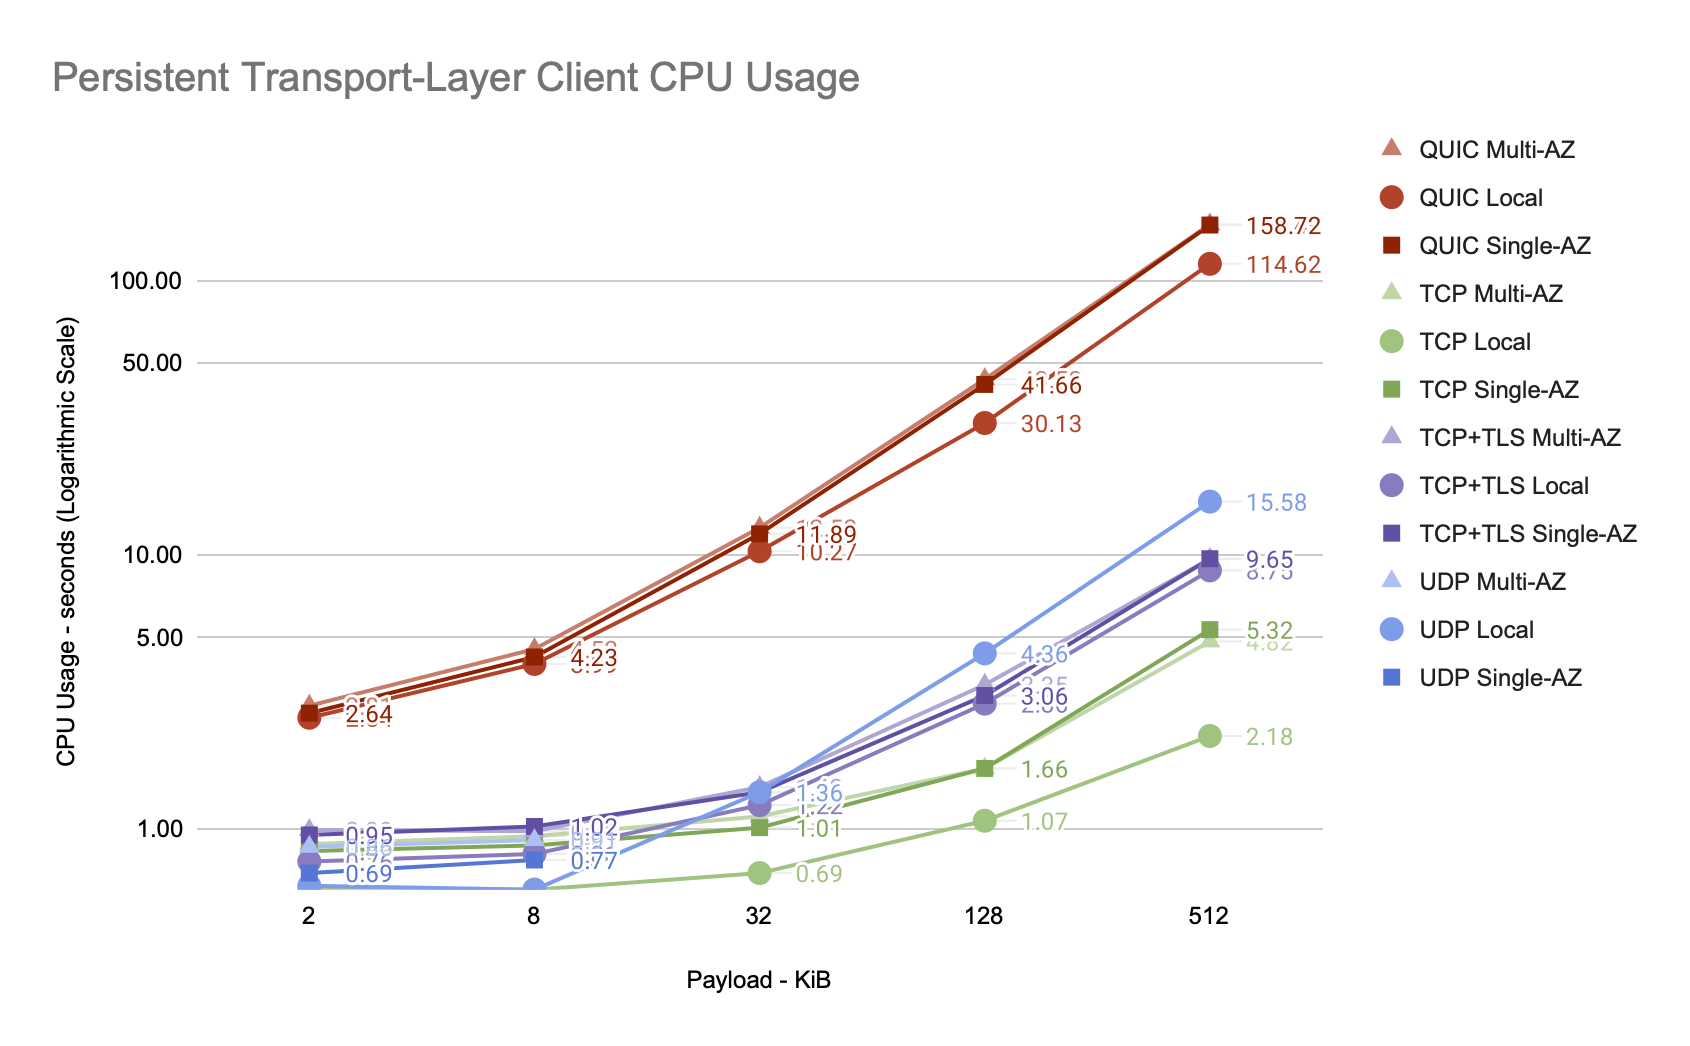
\includegraphics[width=\linewidth]{figures/charts/Persistent Transport-Layer Client CPU Usage.png}
    \caption{Persistent Transport-Layer Client CPU Usage}
    \label{fig:persistent_client_transport_cpu}
\end{figure}

\begin{figure}[h!]
    \centering
    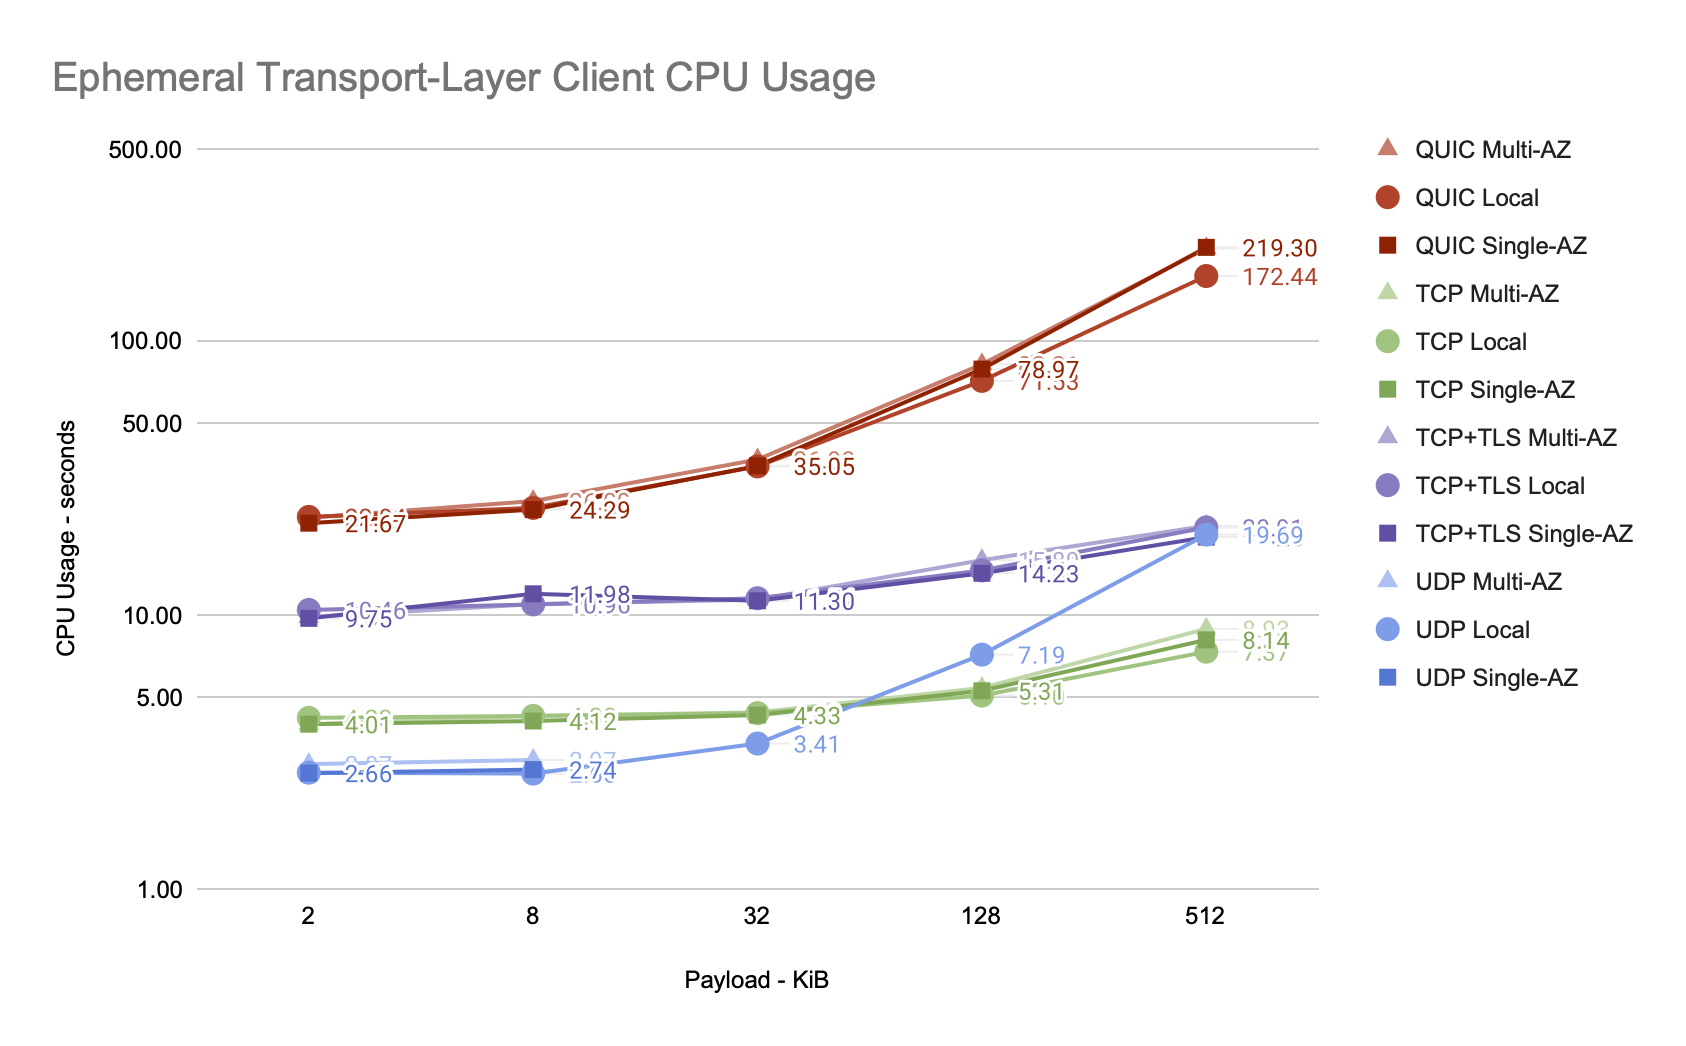
\includegraphics[width=\linewidth]{figures/charts/Ephemeral Transport-Layer Client CPU Usage.png}
    \caption{Ephemeral Transport-Layer Client CPU Usage}
    \label{fig:ephemeral_client_transport_cpu}
\end{figure}

% \begin{figure}[h!]
%     \centering
%     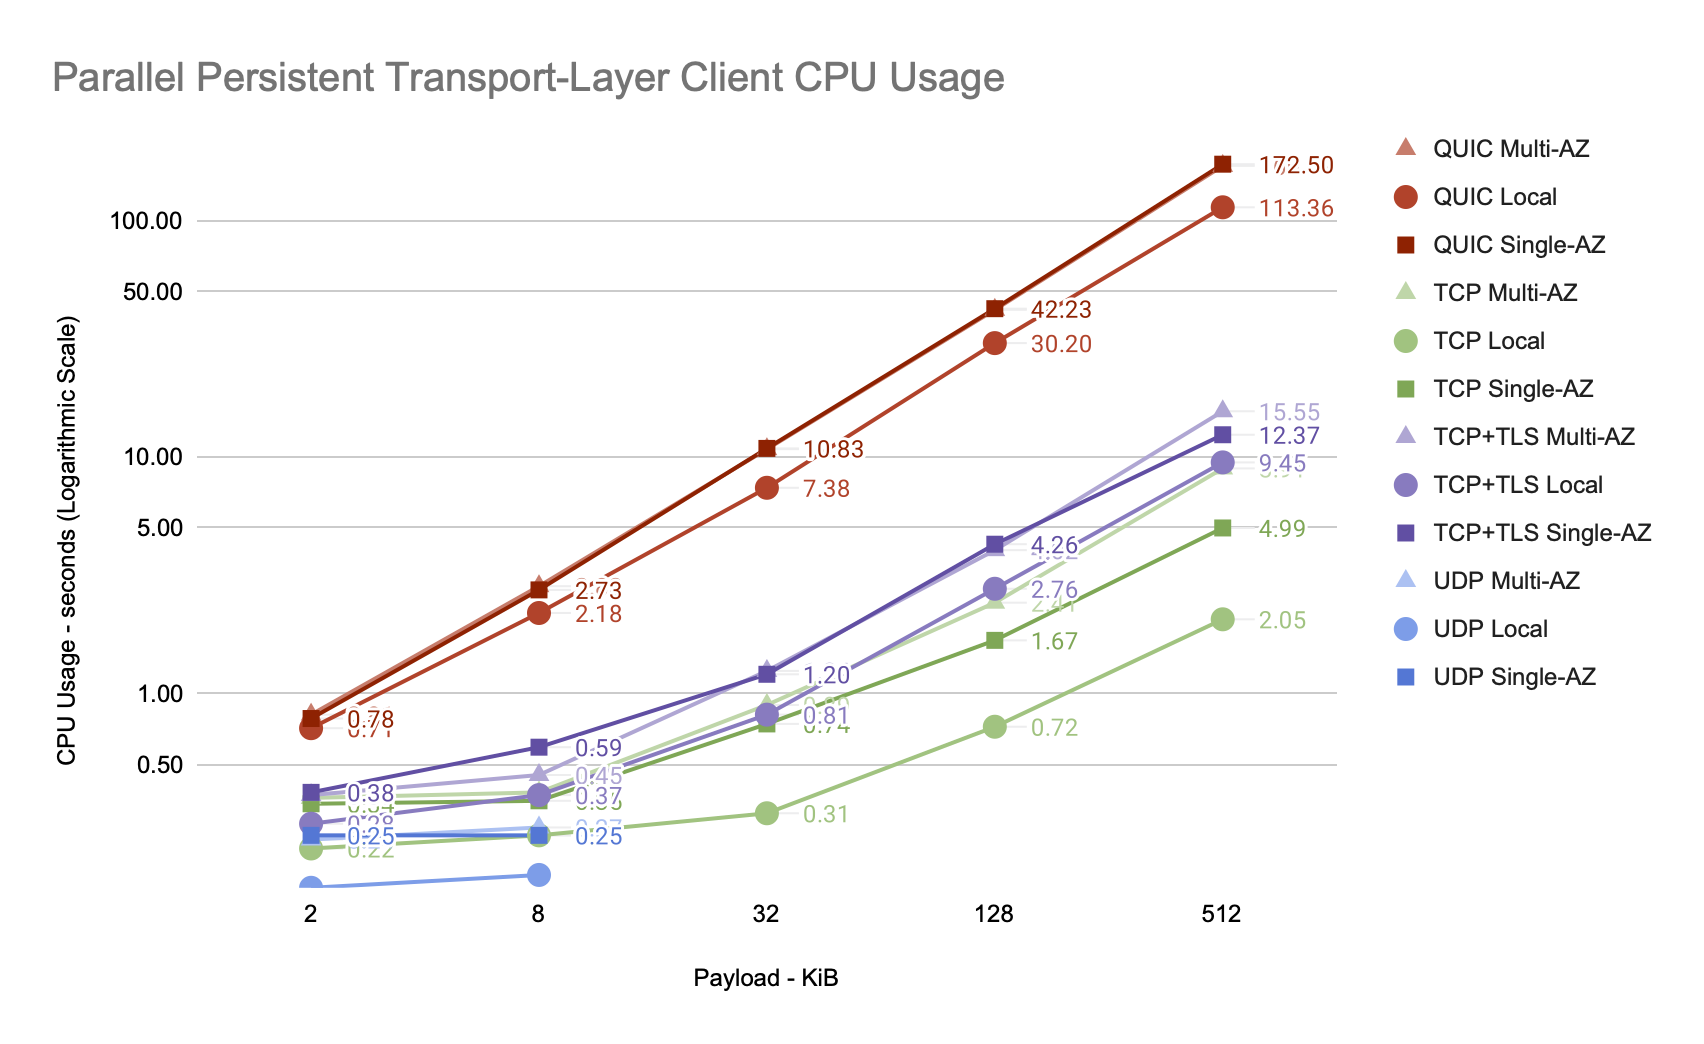
\includegraphics[width=\linewidth]{figures/charts/Parallel Persistent Transport-Layer Client CPU Usage.png}
%     \caption{Parallel Persistent Transport-Layer Client CPU Usage}
%     \label{fig:parallel_client_transport_cpu}
% \end{figure}

\begin{figure}[h!]
    \centering
    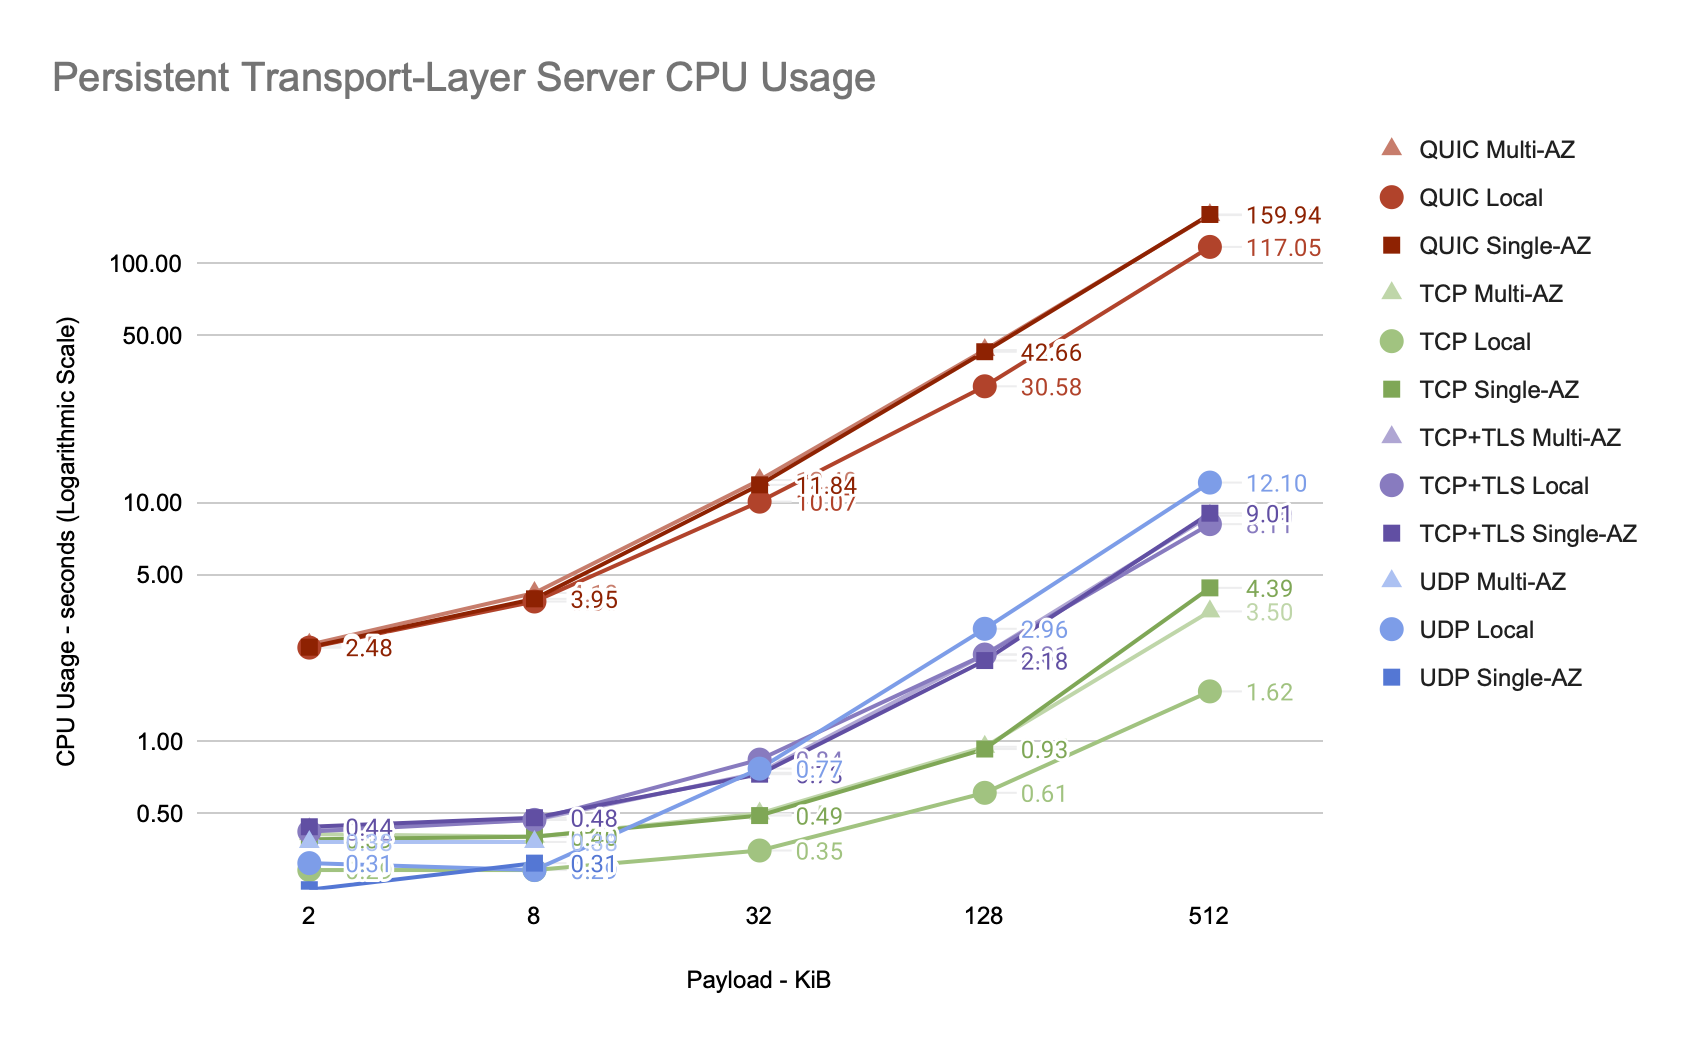
\includegraphics[width=\linewidth]{figures/charts/Persistent Transport-Layer Server CPU Usage.png}
    \caption{Persistent Transport-Layer Server CPU Usage}
    \label{fig:persistent_server_transport_cpu}
\end{figure}

\begin{figure}[h!]
    \centering
    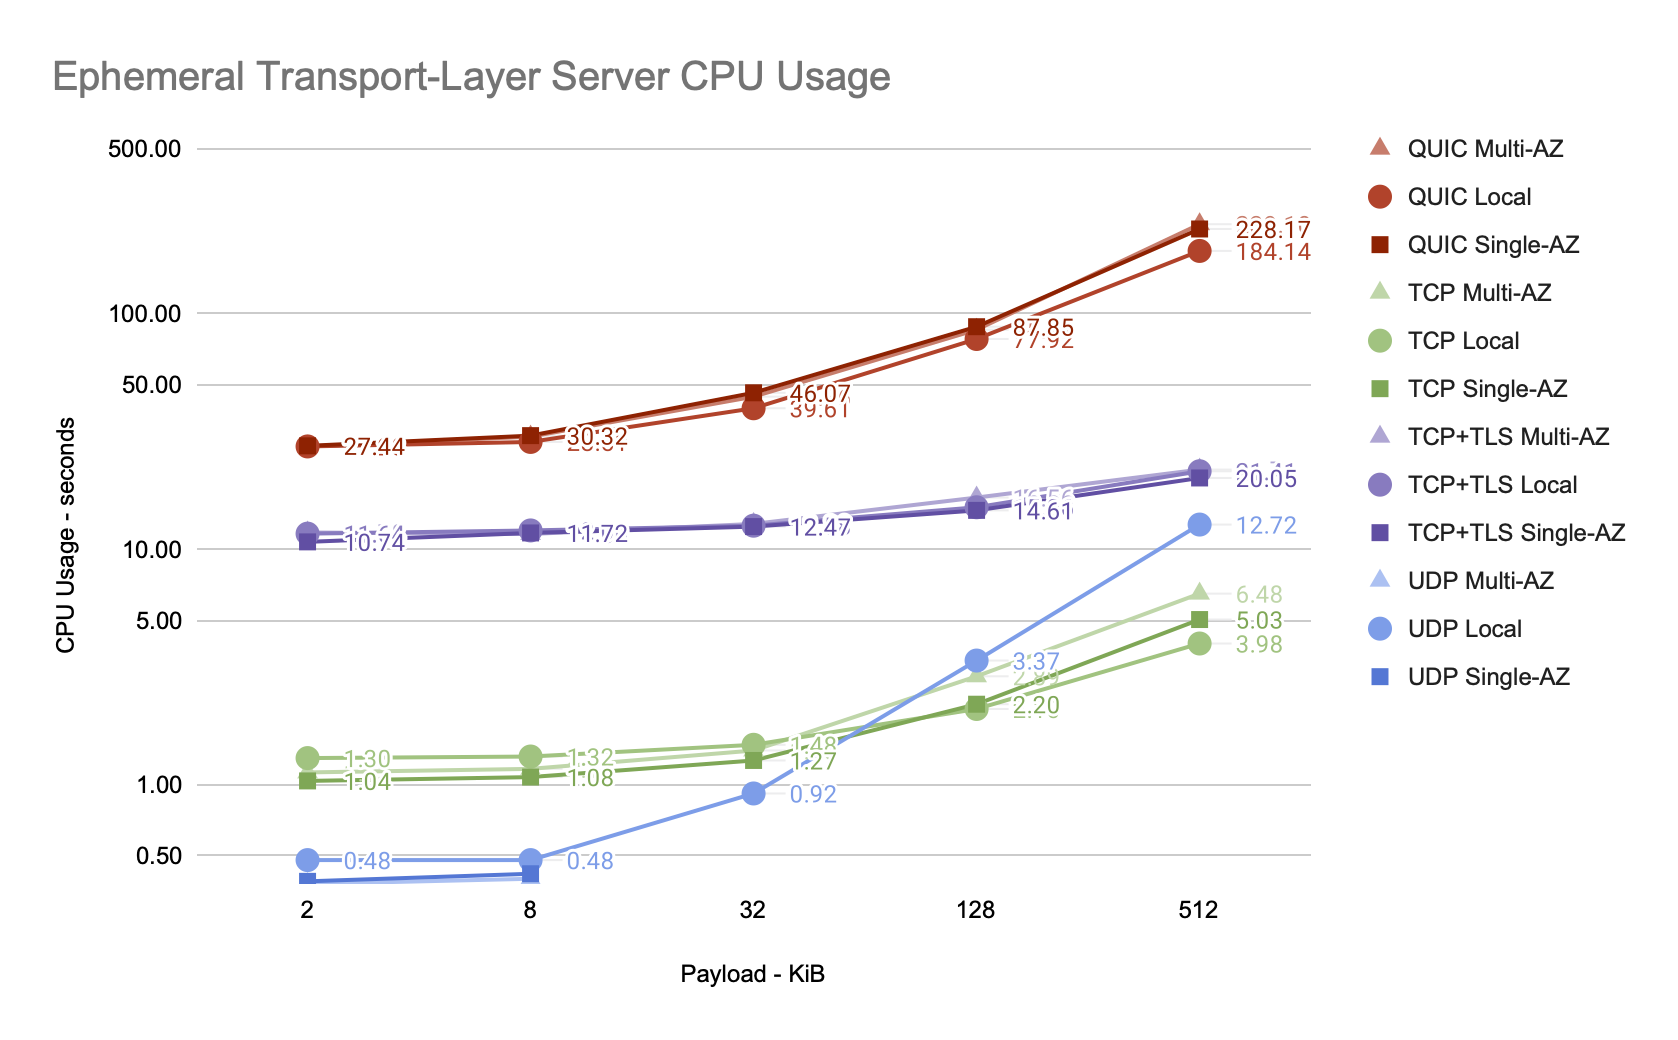
\includegraphics[width=\linewidth]{figures/charts/Ephemeral Transport-Layer Server CPU Usage.png}
    \caption{Ephemeral Transport-Layer Server CPU Usage}
    \label{fig:ephemeral_server_transport_cpu}
\end{figure}

% \begin{figure}[h!]
%     \centering
%     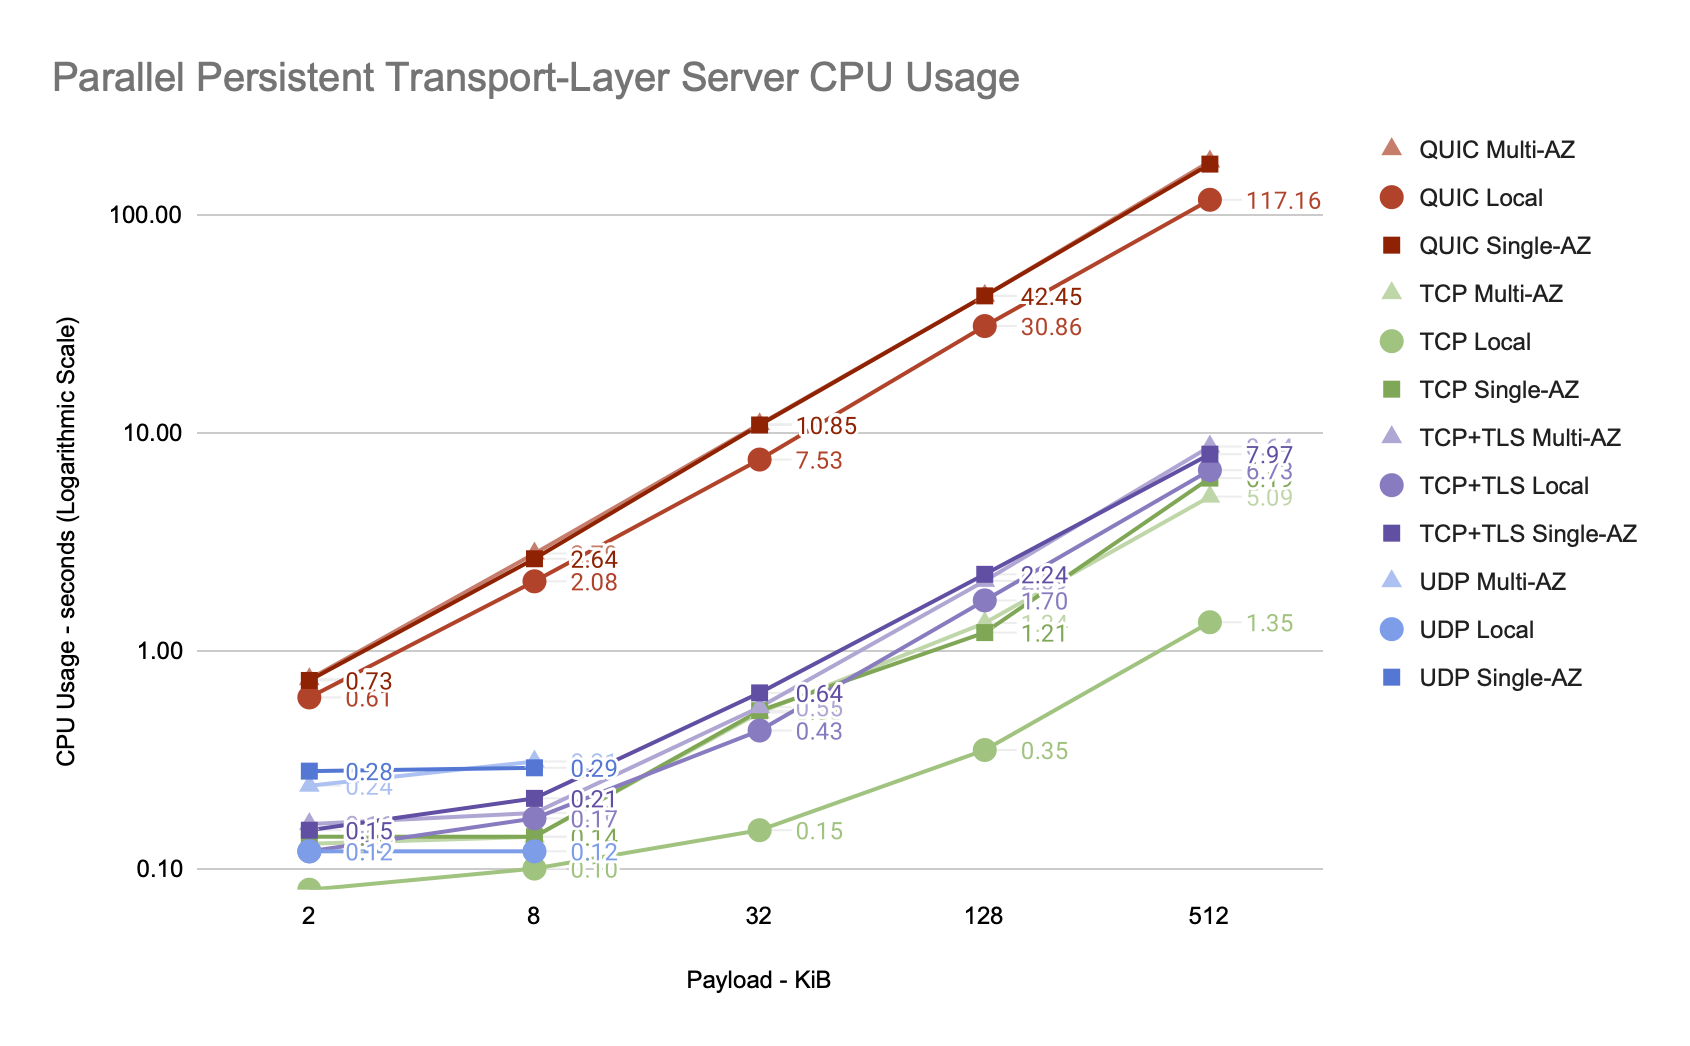
\includegraphics[width=\linewidth]{figures/charts/Parallel Persistent Transport-Layer Server CPU Usage.png}
%     \caption{Parallel Persistent Transport-Layer Server CPU Usage}
%     \label{fig:parallel_server_transport_cpu}
% \end{figure}
